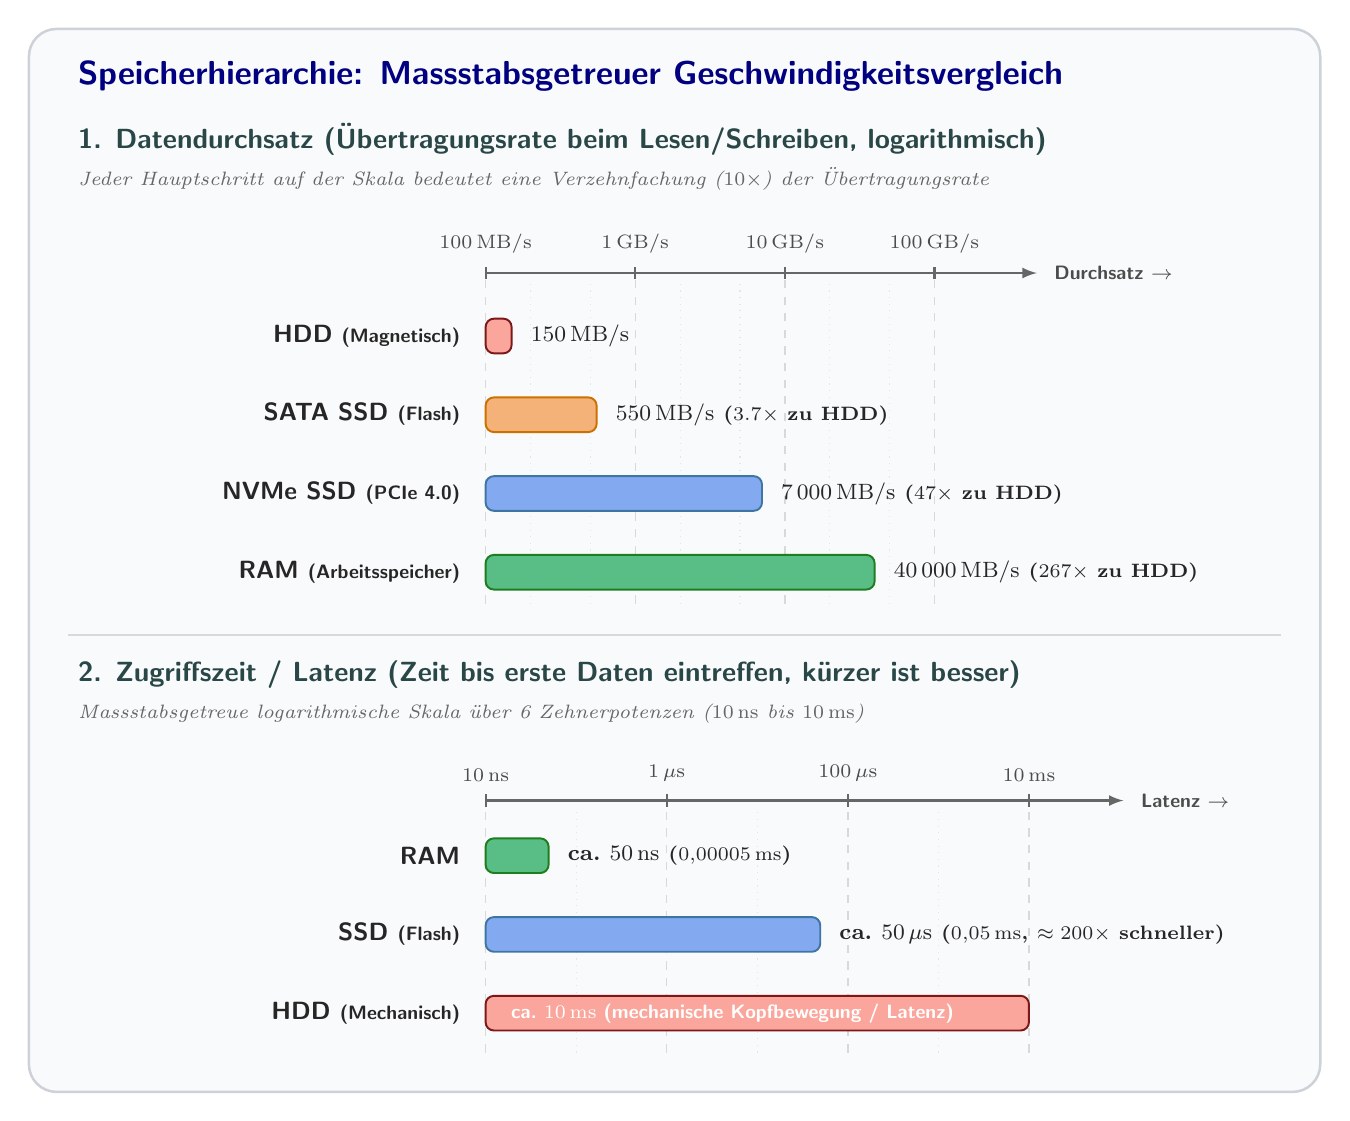
\begin{tikzpicture}[
    font=\small,
    >=latex,
    x=1cm, y=1cm,
    bar/.style={rounded corners=3pt, line width=0.7pt},
    gridline/.style={draw=black!15, dashed, line width=0.5pt},
    labelnode/.style={font=\bfseries\small\sffamily, text=black!85},
    valnode/.style={font=\bfseries\footnotesize, text=black!85}
]

    % Background container (ample padding on left and right)
    \fill[rounded corners=10pt, fill=SlateGray!4, draw=SlateGray!35, line width=0.9pt] (-2.2, -6.6) rectangle (14.2, 6.9);

    % Title
    \node[anchor=west, font=\large\bfseries\sffamily, text=Navy] at (-1.7, 6.3) {Speicherhierarchie: Massstabsgetreuer Geschwindigkeitsvergleich};

    % =========================================================================
    % SECTION 1: DATENDURCHSATZ (Logarithmic Scale)
    % =========================================================================
    \node[anchor=west, font=\bfseries\normalsize\sffamily, text=DarkSlateGray!90!black] at (-1.7, 5.5) {1. Datendurchsatz (Übertragungsrate beim Lesen/Schreiben, logarithmisch)};
    \node[anchor=west, font=\itshape\scriptsize, text=black!60] at (-1.7, 5.0) {Jeder Hauptschritt auf der Skala bedeutet eine Verzehnfachung ($10\times$) der Übertragungsrate};

    % Log Scale: x(v) = 3.60 + 1.90 * log10(v / 100)
    % 100 MB/s    -> 3.60
    % 1 GB/s      -> 5.50
    % 10 GB/s     -> 7.40
    % 100 GB/s    -> 9.30

    % Gridlines & Major Ticks
    \draw[gridline] (3.60, -0.4) -- (3.60, 3.8);
    \draw[gridline] (5.50, -0.4) -- (5.50, 3.8);
    \draw[gridline] (7.40, -0.4) -- (7.40, 3.8);
    \draw[gridline] (9.30, -0.4) -- (9.30, 3.8);

    % Minor gridlines (dotted)
    \foreach \x in {4.17, 4.93, 6.07, 6.83, 7.97, 8.73} {
        \draw[draw=black!10, dotted, line width=0.4pt] (\x, -0.4) -- (\x, 3.7);
    }

    % Axis Line with ticks
    \draw[->, thick, color=black!60] (3.6, 3.8) -- (10.6, 3.8);
    \node[anchor=west, font=\scriptsize\bfseries\sffamily, text=black!70] at (10.7, 3.8) {Durchsatz $\rightarrow$};

    \foreach \x/\lbl in {3.60/{100\,\mathrm{MB/s}}, 5.50/{1\,\mathrm{GB/s}}, 7.40/{10\,\mathrm{GB/s}}, 9.30/{100\,\mathrm{GB/s}}} {
        \draw[black!60, line width=0.8pt] (\x, 3.72) -- (\x, 3.88);
        \node[anchor=south, font=\scriptsize\bfseries, text=black!70] at (\x, 3.92) {$\lbl$};
    }

    % HDD Bar: 150 MB/s -> 3.60 + 1.90*log10(1.5) = 3.93
    \node[anchor=east, labelnode] at (3.4, 3.0) {HDD \scriptsize(Magnetisch)};
    \fill[bar, fill=Salmon!70, draw=FireBrick!70!black] (3.60, 2.78) rectangle (3.93, 3.22);
    \node[anchor=west, valnode] at (4.05, 3.0) {$150\,\mathrm{MB/s}$};

    % SATA SSD Bar: 550 MB/s -> 3.60 + 1.90*log10(5.5) = 5.01
    \node[anchor=east, labelnode] at (3.4, 2.0) {SATA SSD \scriptsize(Flash)};
    \fill[bar, fill=SandyBrown!85, draw=DarkOrange!80!black] (3.60, 1.78) rectangle (5.01, 2.22);
    \node[anchor=west, valnode] at (5.13, 2.0) {$550\,\mathrm{MB/s}$ \scriptsize(\textbf{$3.7\times$} zu HDD)};

    % NVMe SSD Bar: 7000 MB/s -> 3.60 + 1.90*log10(70) = 7.11
    \node[anchor=east, labelnode] at (3.4, 1.0) {NVMe SSD \scriptsize(PCIe 4.0)};
    \fill[bar, fill=CornflowerBlue!80, draw=SteelBlue!90!black] (3.60, 0.78) rectangle (7.11, 1.22);
    \node[anchor=west, valnode] at (7.23, 1.0) {$7\,000\,\mathrm{MB/s}$ \scriptsize(\textbf{$47\times$} zu HDD)};

    % RAM Bar: 40000 MB/s -> 3.60 + 1.90*log10(400) = 8.54
    \node[anchor=east, labelnode] at (3.4, 0.0) {RAM \scriptsize(Arbeitsspeicher)};
    \fill[bar, fill=MediumSeaGreen!85, draw=ForestGreen!90!black] (3.60, -0.22) rectangle (8.54, 0.22);
    \node[anchor=west, valnode] at (8.66, 0.0) {$40\,000\,\mathrm{MB/s}$ \scriptsize(\textbf{$267\times$} zu HDD)};


    % =========================================================================
    % SECTION 2: ZUGRIFFSZEIT / LATENZ (Logarithmic Scale)
    % =========================================================================
    \draw[thick, color=black!15] (-1.7, -0.8) -- (13.7, -0.8);
    \node[anchor=west, font=\bfseries\normalsize\sffamily, text=DarkSlateGray!90!black] at (-1.7, -1.3) {2. Zugriffszeit / Latenz (Zeit bis erste Daten eintreffen, kürzer ist besser)};
    \node[anchor=west, font=\itshape\scriptsize, text=black!60] at (-1.7, -1.8) {Massstabsgetreue logarithmische Skala über 6 Zehnerpotenzen ($10\,\mathrm{ns}$ bis $10\,\mathrm{ms}$)};

    % Latency Scale: 6 decades from 10ns to 10ms -> 1.15 cm per decade
    % x(t) = 3.60 + 1.15 * log10(t / 10ns)
    % 10 ns   -> 3.60
    % 100 ns  -> 4.75
    % 1 us    -> 5.90
    % 10 us   -> 7.05
    % 100 us  -> 8.20
    % 1 ms    -> 9.35
    % 10 ms   -> 10.50

    % Gridlines for latency
    \draw[gridline] (3.60, -6.1) -- (3.60, -2.9);
    \draw[gridline] (5.90, -6.1) -- (5.90, -2.9);
    \draw[gridline] (8.20, -6.1) -- (8.20, -2.9);
    \draw[gridline] (10.50, -6.1) -- (10.50, -2.9);

    % Minor gridlines for latency
    \foreach \x in {4.75, 7.05, 9.35} {
        \draw[draw=black!10, dotted, line width=0.4pt] (\x, -6.1) -- (\x, -3.0);
    }

    % Axis line with ticks
    \draw[->, thick, color=black!60] (3.6, -2.9) -- (11.7, -2.9);
    \node[anchor=west, font=\scriptsize\bfseries\sffamily, text=black!70] at (11.8, -2.9) {Latenz $\rightarrow$};

    \foreach \x/\lbl in {3.60/{10\,\mathrm{ns}}, 5.90/{1\,\mu\mathrm{s}}, 8.20/{100\,\mu\mathrm{s}}, 10.50/{10\,\mathrm{ms}}} {
        \draw[black!60, line width=0.8pt] (\x, -2.98) -- (\x, -2.82);
        \node[anchor=south, font=\scriptsize\bfseries, text=black!70] at (\x, -2.78) {$\lbl$};
    }

    % RAM Latency: 50 ns -> 3.60 + 1.15*log10(5) = 4.40
    \node[anchor=east, labelnode] at (3.4, -3.6) {RAM};
    \fill[bar, fill=MediumSeaGreen!85, draw=ForestGreen!90!black] (3.60, -3.82) rectangle (4.40, -3.38);
    \node[anchor=west, valnode] at (4.52, -3.6) {ca.\ $50\,\mathrm{ns}$ \scriptsize($0{,}00005\,\mathrm{ms}$)};

    % SSD Latency: 50 us -> 3.60 + 1.15*log10(5000) = 7.85
    \node[anchor=east, labelnode] at (3.4, -4.6) {SSD \scriptsize(Flash)};
    \fill[bar, fill=CornflowerBlue!80, draw=SteelBlue!90!black] (3.60, -4.82) rectangle (7.85, -4.38);
    \node[anchor=west, valnode] at (7.97, -4.6) {ca.\ $50\,\mu\mathrm{s}$ \scriptsize($0{,}05\,\mathrm{ms}$, \textbf{$\approx 200\times$} schneller)};

    % HDD Latency: 10 ms (10^7 ns) -> 3.60 + 1.15*6 = 10.50
    \node[anchor=east, labelnode] at (3.4, -5.6) {HDD \scriptsize(Mechanisch)};
    \fill[bar, fill=Salmon!70, draw=FireBrick!70!black] (3.60, -5.82) rectangle (10.50, -5.38);
    % Inset label inside bar
    \node[anchor=west, font=\bfseries\scriptsize\sffamily, text=white] at (3.80, -5.6) {ca.\ $10\,\mathrm{ms}$ (mechanische Kopfbewegung / Latenz)};

\end{tikzpicture}
